\documentclass{sydeStyle}
\usepackage{booktabs}
\usepackage{graphicx}
\usepackage{multirow}
\usepackage{tabularx}

\title{Lab 1: Clusters and Classification Boundaries}
\coursecode{372}
\author{
    David Kadish, 20176757\\
    Zhao Peng, 20326604\\
    Matt Stewart, 20205320\\
}
\prof{Professor P. Fieguth}
\date{February 9, 2009}

\begin{document}

\pagenumbering{roman}

\maketitle

\setcounter{page}{2} % the table of contents will be shown as page iii

\pagenumbering{arabic}

\chapter{Introduction}
The purpose of this lab was to apply pattern recognition classification
algorithms and concepts to data sets in Matlab.  Parameters such  as
number of data points, means, covariance matrices,  and number of clustes  were
given.  Randomized clusters were generated based on the class 
specifications, forming classification boundaries, and determining the
probability of error based on those classification boundaries.


\chapter{Implementation}
The implementation for Lab 1 is done using MATLAB's class structures to
maximize the reusability and allow for experiementation beyond the requirements
of the lab. This is discussed further in Chapter \ref{cha:results}.

\section{Classes}
MATLAB classes were created for parametric and non-parametric classifiers. The
classes, {\tt ParametricClass} and {\tt NonParametricClass} are presented in
Appendix \ref{cha:code}.
\subsection{Properties and class functions}
The two classes store properties related to the pattern recognition problems
they represent. The {\tt ParametricClass} stores for a class $A$ the values of
$\mu_A$, $\Sigma_A$ and $p(A)$. The {\tt NonParametricClass} stores a cluster
of $n$ points in a Gaussian distribution with the parameters $\mu$
and $\Sigma$.

Each class provides methods for calculating the various distance measures
associated with the type of problem that it represents. The {\tt
ParametricClass} has functions for calculating $d^2$ using both MED and GED as
well as a function for calculating the value of $p(A) \cdot p(x|A)$ as a
measure of probability for MAP classification. The {\tt NonParametricClass} contains a
function for calculating distance to the class using kNN.

The classes also provide helper functions for creating graphical
representations of their data. {\tt
ParametricClass}

\subsection{Static methods}

\section{Helper functions}
\subsection{Tools}
\subsection{Plot ellipse}

\section{Main file}
\includegraphics{test}

\chapter{Results}
\label{cha:results}
\section{Cluster Generation}
%1.	Visually, how does the unit contour relate to the cluster data?
The unit contour represents a collection of equally likely points in space. 
The elliptical unit standard deviation contours match the rough elliptical 
shape of the data clusters. The unit standard deviation contour does not 
enclose all data points.  This is expected as the random data 
points that make up the clusters were generated on a normal distribution with 
a given mean and covariance; we would not expect all data points to be within 
one standard deviation of the mean.

\section{Classification Boundaries}
%2.	Comment on the classification boundaries. How do the different boundaries
%compare?

\subsection{Parametric}

\begin{figure}
  \begin{center}
  	\label{fig:2param}  
    \caption{The clusters, unit standard deviation curves and
    parametric classification boundaries for the 2 class case.}
    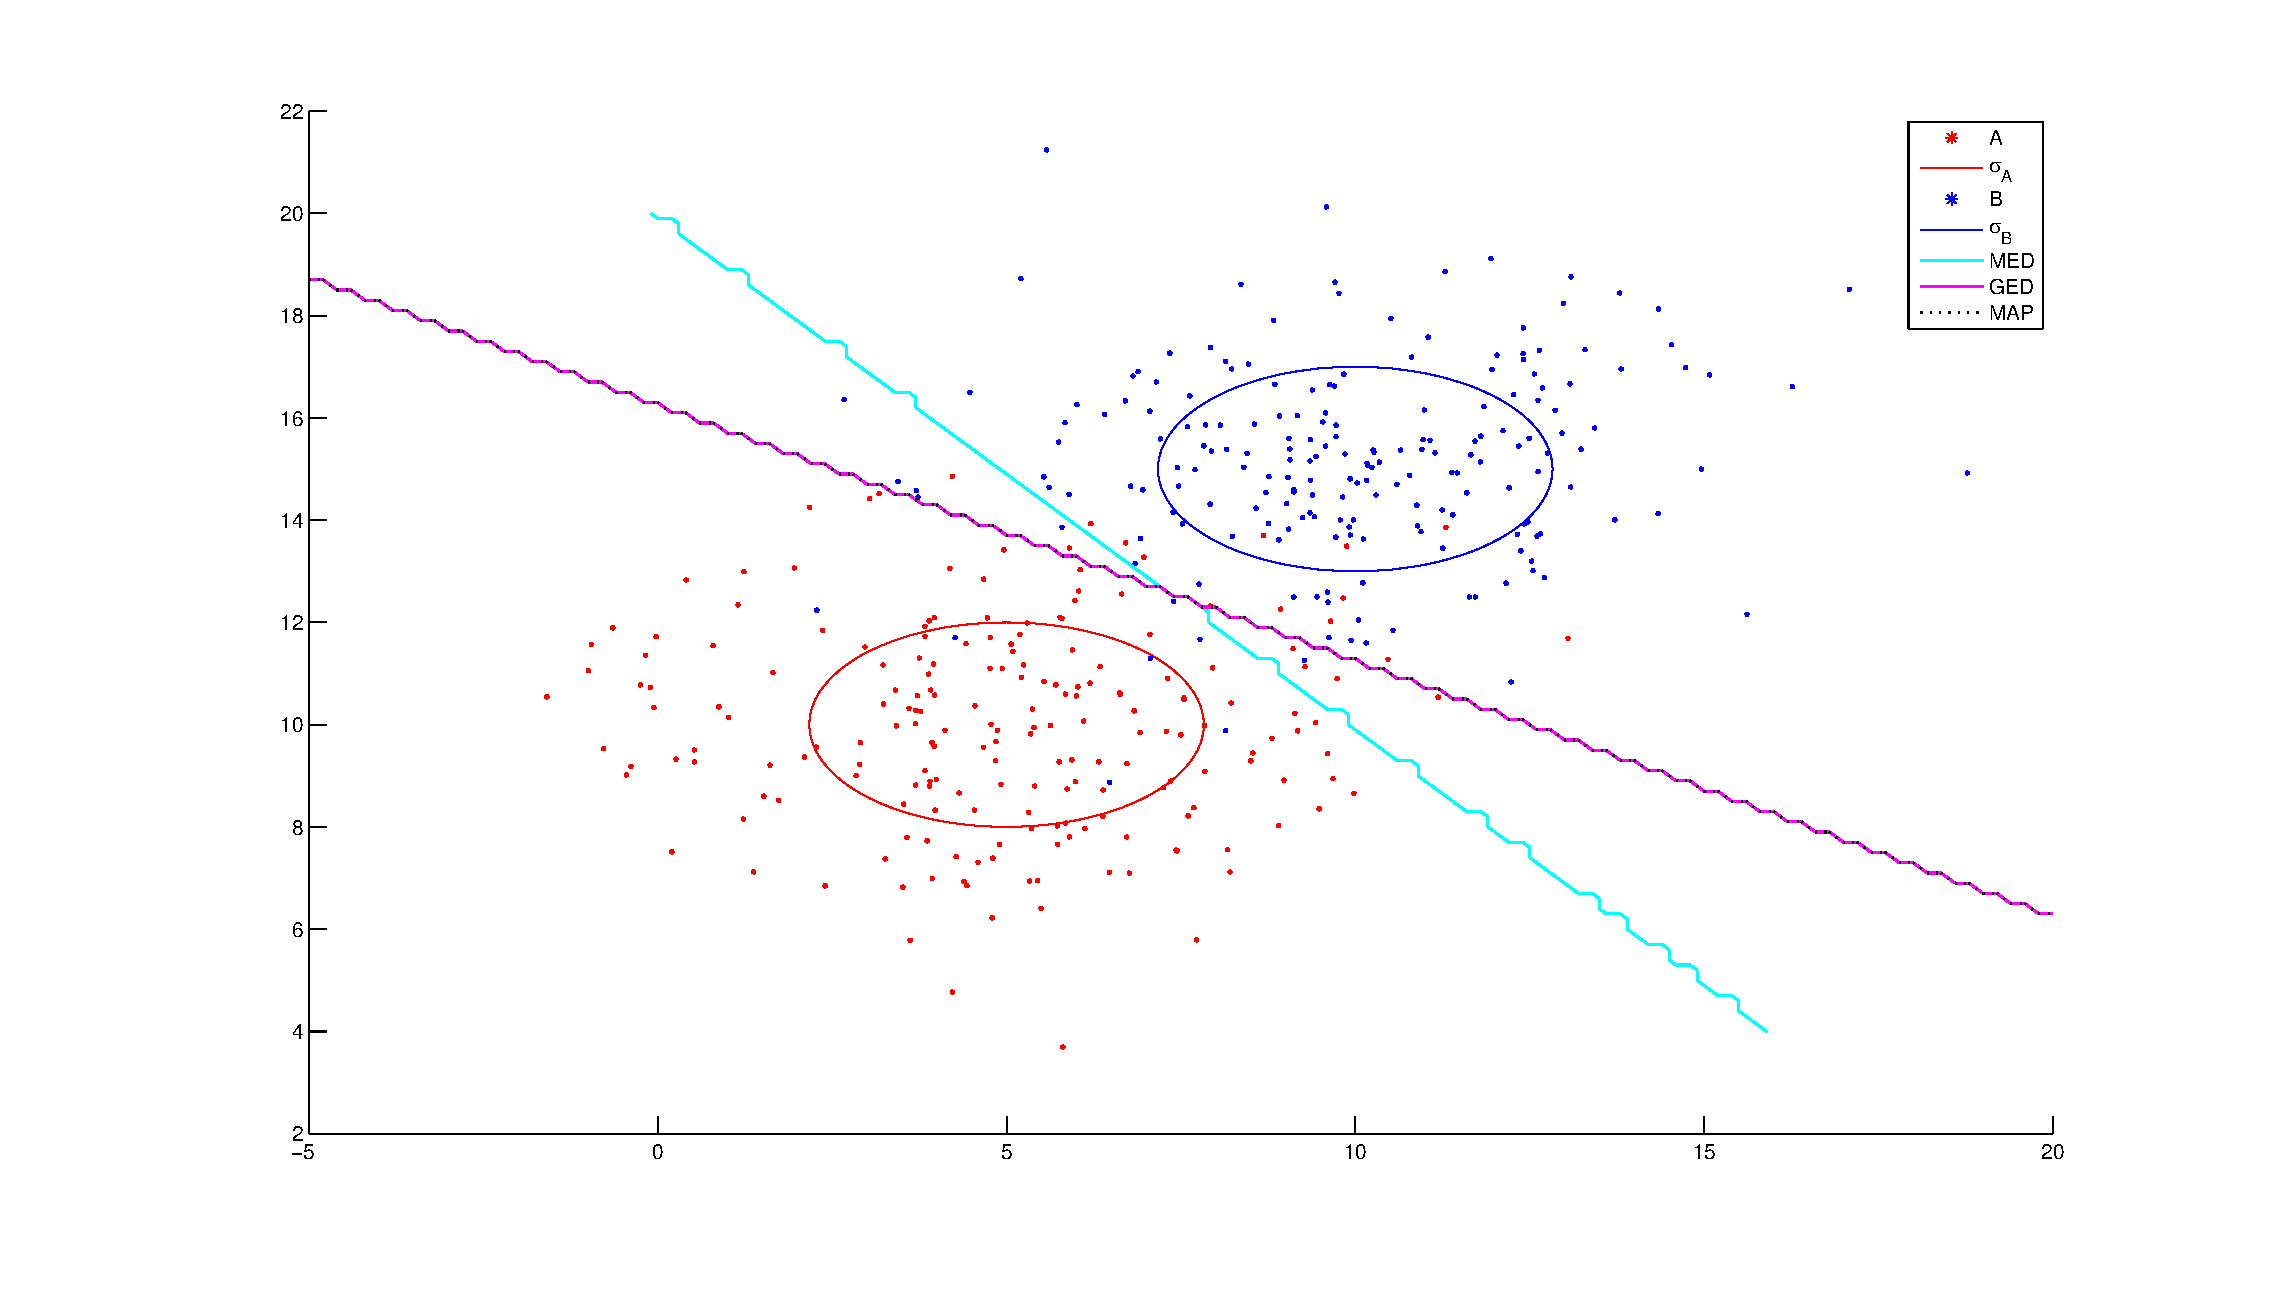
\includegraphics[width=15cm]{figures/2-param}
  \end{center}
\end{figure}

\begin{figure}
  \begin{center}
  	\label{fig:3param}
    \caption{The clusters, unit standard deviation curves and
    parametric classification boundaries for the 3 class case.}
    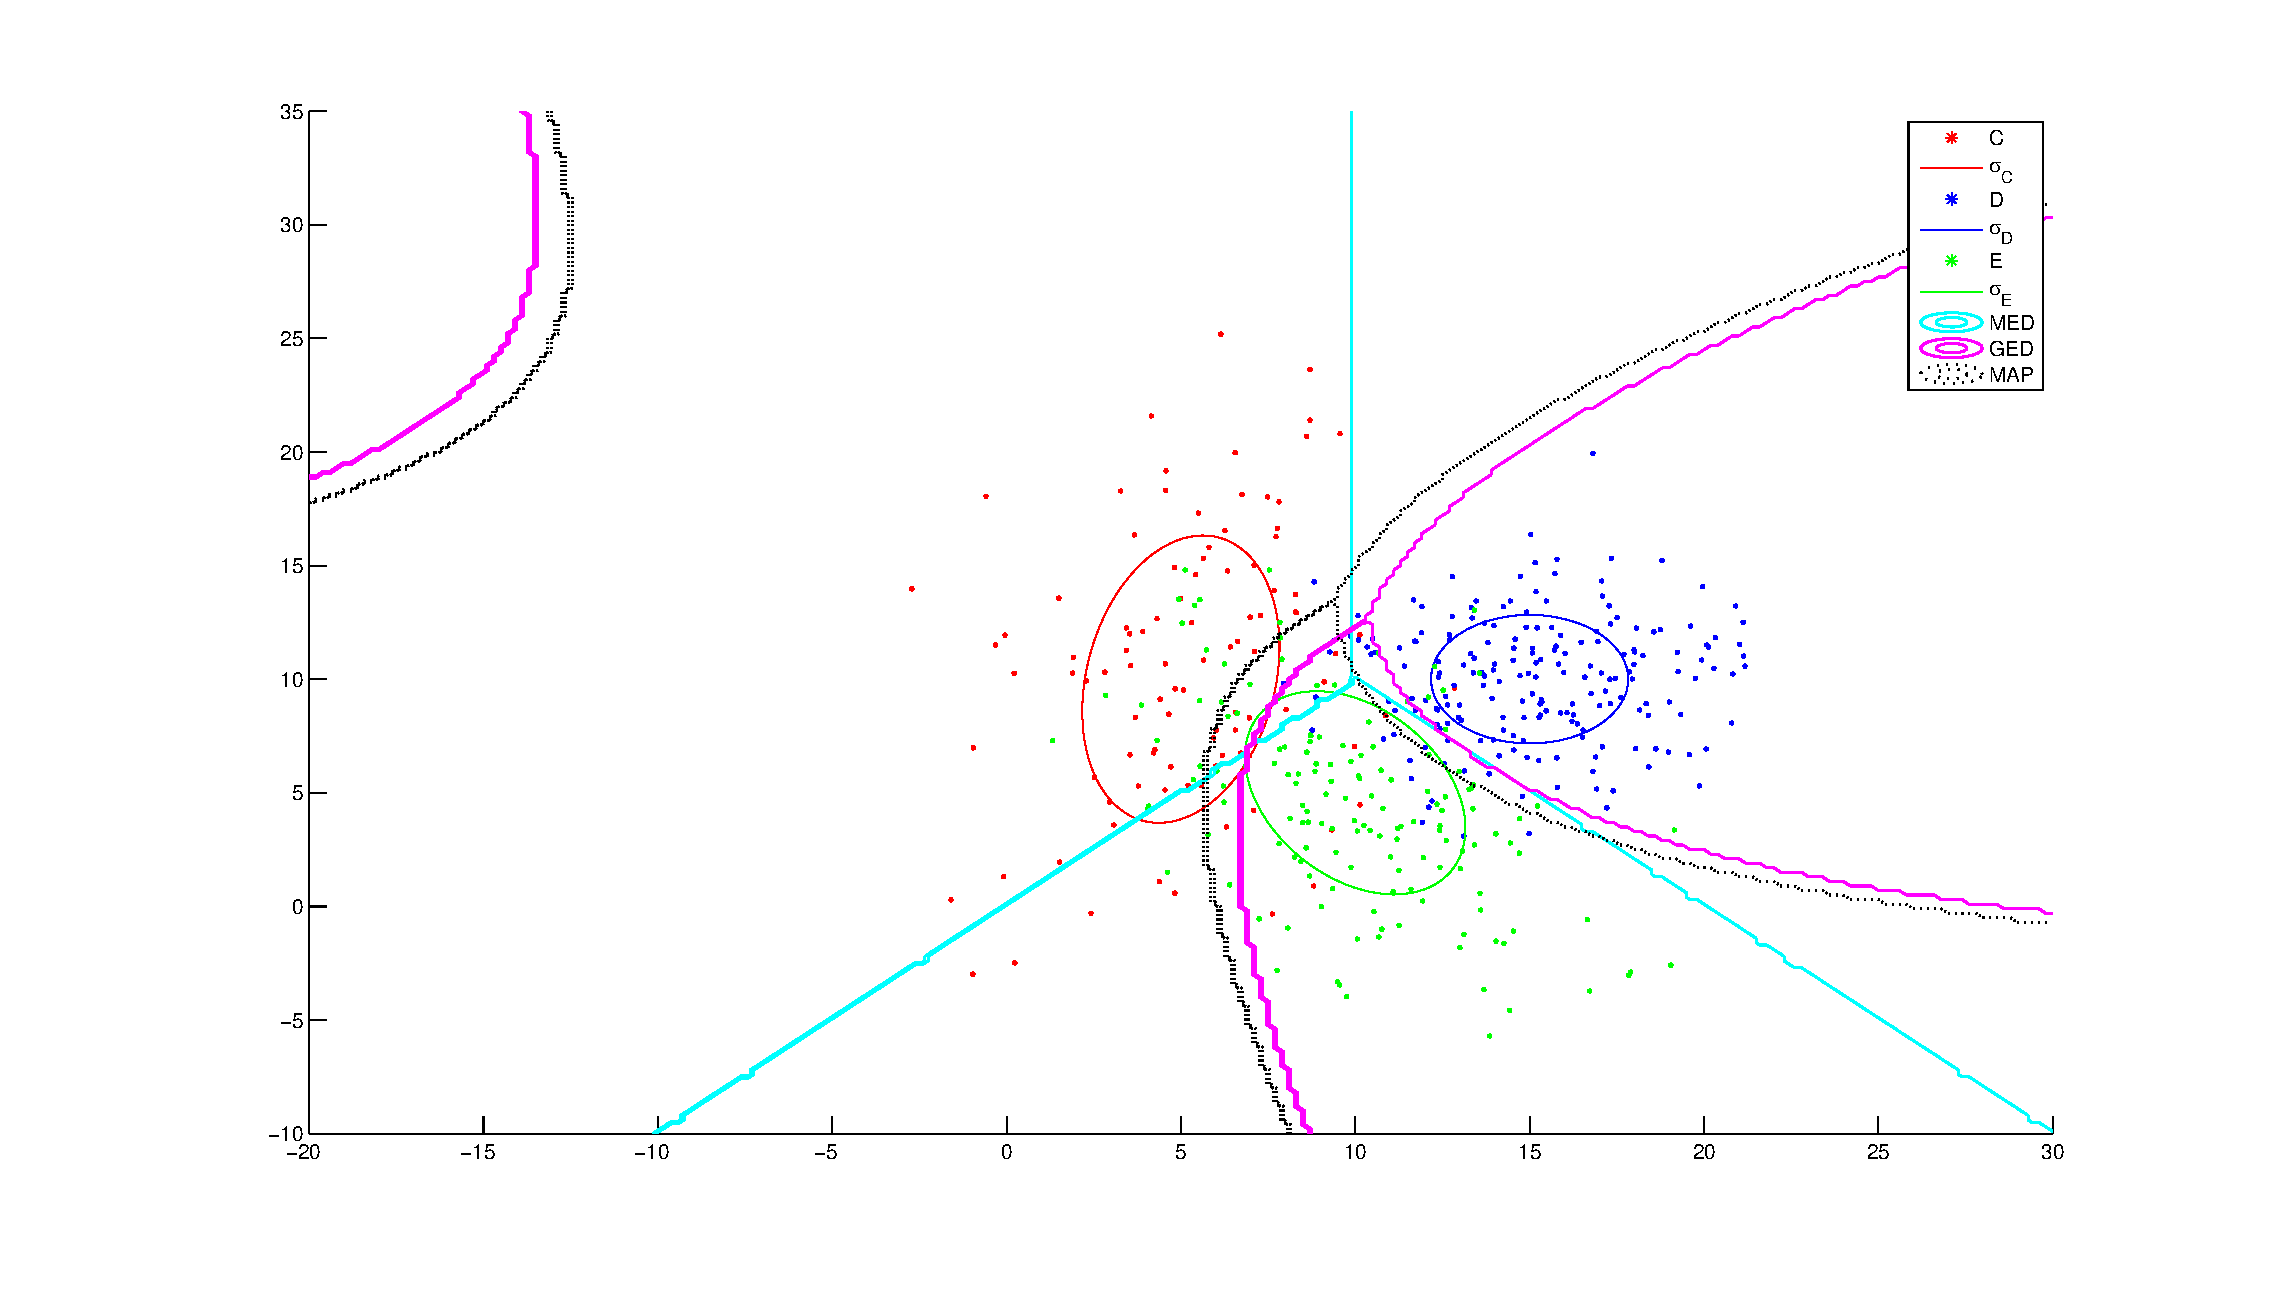
\includegraphics[width=15cm]{figures/3-param}
  \end{center}
\end{figure}

Figure \ref{fig:2param} demonstrates how the GED classifier 
was better than MED in the 2 class case.  The MED classifier
does not take the shape of the cluster (ie. the variances) into account and
relies solely on the location of the cluster mean. GED, on the
other hand, accounts for the variances and therefore generates a rotated
classifier. In the 2 class case, the GED and MAP classifiers generate the same
boundary because the variances of the two classes are equal.

The 3 class case in Figure \ref{fig:3param} demonstrates the relative strength
of the MAP method. The MED boundary is simply an intersecting set of straight
lines reflecting the points equidistant from the closest class averages. The
GED and MAP boundaries have the same basic shape, but the MAP boundary provides
a narrower avenue where it would classify a point as C or E. This reflects the
relatively high value of $P(D)$ in the space.

\subsection{Non-parametric}

\begin{figure}
  \begin{center}
  	\label{fig:2nonparam}  
    \caption{The clusters and non-parametric classification
    boundaries for the 2 class case.}
    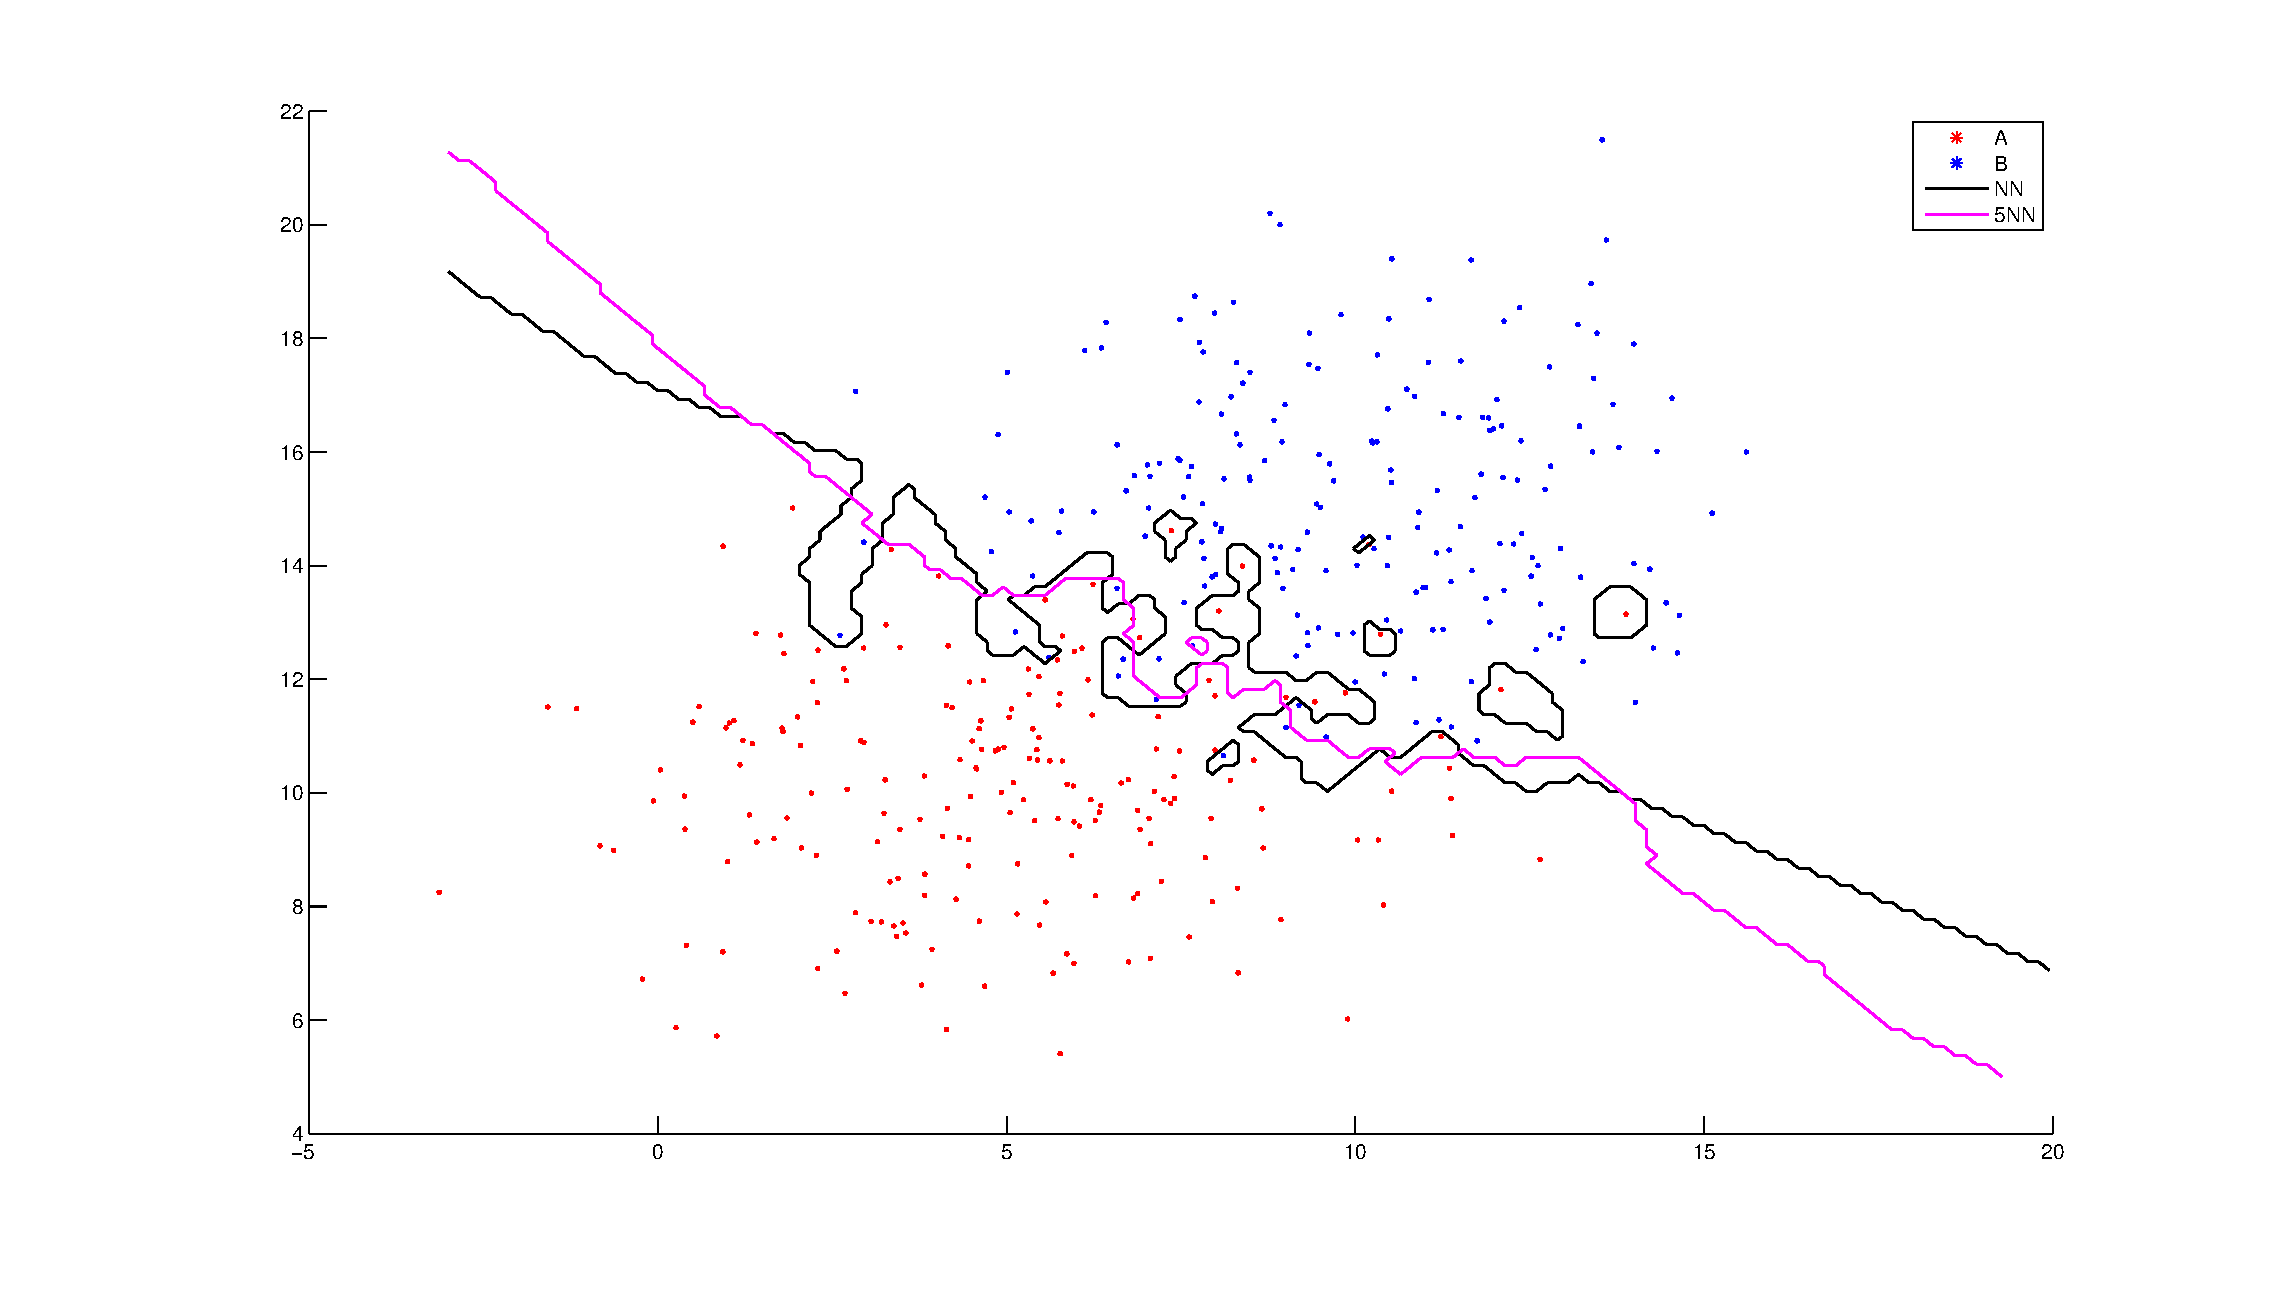
\includegraphics[width=15cm]{figures/2-nonparam}
  \end{center}
\end{figure}

\begin{figure}
  \begin{center}
  	\label{fig:3nonparam}
    \caption{The clusters and non-parametric classification
    boundaries for the 3 class case.}
    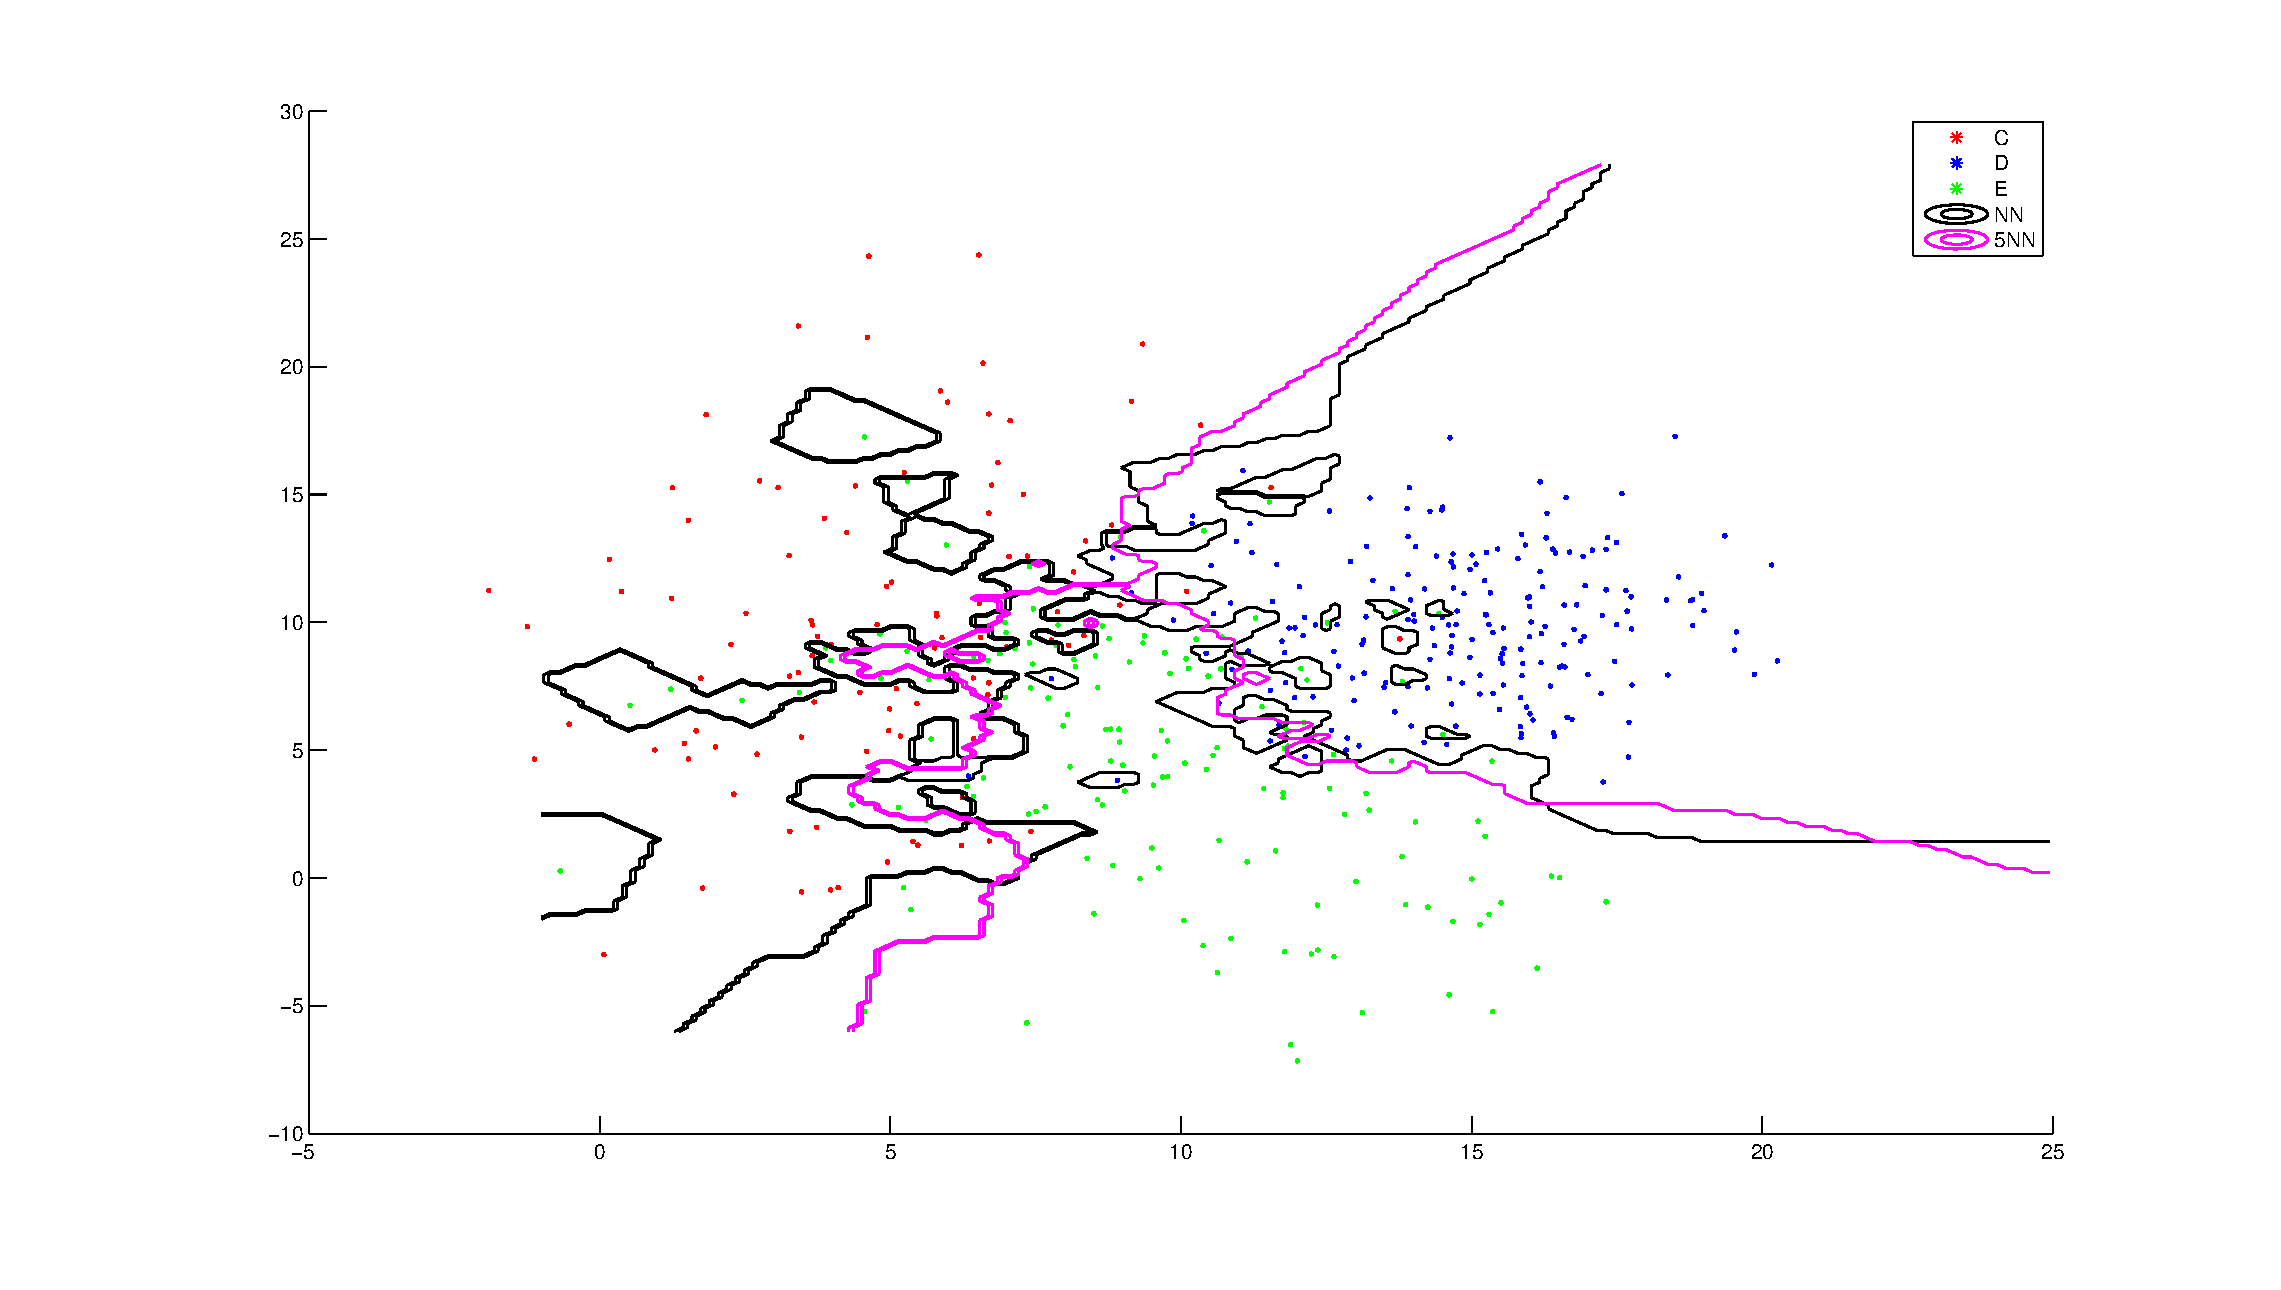
\includegraphics[width=15cm]{figures/3-nonparam}
  \end{center}
\end{figure}

The 5NN classifier displays a much simpler 
boundary than the NN classifier.  The key distinction is the fact that the 5NN is  less sensitive to 
outliers because it ignores the four nearest points from each class.
NN differs from 5NN in two major ways: Firstly, the NN classifier has more individual boundaries. Secondly, these boundaries are much 
less smooth than 5NN.

It is interesting to note in both the 2- and 3-class cases that the kNN
boundary is beginning to look similar to the MAP boundary for the parametric
class with the same $\mu$ and $\Sigma$ as $k$ goes from 1 to 5.

\section{Error Anaylsis}
%3.	Compare the results. Which error is smallest? What do you observe in the
%confusion matrices for CASE2?

\begin{table}[h]
\centering
\caption{Confusion matrix and probability of error for the 2 class case}
\label{tab:conf2class}
\vspace{6pt}
\begin{tabular}{lcccc}
\toprule
 & \multicolumn{2}{c}{Test 1} & \multicolumn{2}{c}{Test 2} \\
\cmidrule(r){2-3} \cmidrule(r){4-5}
 & $M_{confusion}$ & $P(\varepsilon)$ & $M_{confusion}$ & $P(\varepsilon)$ \\
\midrule
MED &
\begin{bmatrix}
   188 &   15 \\
    12 &  185 \\
\end{bmatrix}
& 0.0675 &
\begin{bmatrix}
   182 &   22\\
    18 &  178\\
\end{bmatrix}
& 0.1000\\\addlinespace
GED &
\begin{bmatrix}
   190 &   17\\
    10 &  183\\
\end{bmatrix}
& 0.0675 &
\begin{bmatrix}
   186 &   18\\
    14 &  182\\
\end{bmatrix}
& 0.0800 \\\addlinespace
MAP &
\begin{bmatrix}
   190 &   17\\
    10 &  183\\
\end{bmatrix}
& 0.0675 &
\begin{bmatrix}
   186 &   18\\
    14 &  182\\
\end{bmatrix}
& 0.0800	\\	\addlinespace
NN &
\begin{bmatrix}
   175 &   22\\
    25 &  178\\
\end{bmatrix}
& 0.1175 &
\begin{bmatrix}
   178 &   27\\
    22 &  173\\
\end{bmatrix}
& 0.1225	\\	\addlinespace
5NN &
\begin{bmatrix}
   187 &   16\\
    13 &  184\\
\end{bmatrix}
& 0.0725 &
\begin{bmatrix}
   187 &   23\\
    13 &  177\\
\end{bmatrix}
& 0.0900	\\
\bottomrule
\end{tabular}
\end{table}

\begin{table}[h]
\centering
\caption{Confusion matrix and probability of error for the 3 class case}
\label{tab:conf3class}
\vspace{6pt}
\begin{tabular}{lcccc}
\toprule
 & \multicolumn{2}{c}{Test 1} & \multicolumn{2}{c}{Test 2} \\
\cmidrule(r){2-3} \cmidrule(r){4-5}
 & $M_{confusion}$ & $P(\varepsilon)$ & $M_{confusion}$ & $P(\varepsilon)$ \\
\midrule
MED &
\begin{bmatrix}
    78 &    1 &   29\\
     4 &  183 &   16\\
    18 &   16 &  105\\
\end{bmatrix}
& 0.1867 &
\begin{bmatrix}
    80 &    4 &   22\\
     2 &  175 &   21\\
    18 &   21 &  107\\
\end{bmatrix}
& 0.1956\\\addlinespace
GED &
\begin{bmatrix}
    94 &    3 &   36\\
     2 &  174 &   11\\
     4 &   23 &  103\\
\end{bmatrix}
& 0.1756 &
\begin{bmatrix}
    89 &    1 &   28\\
     0 &  170 &   18\\
    11 &   29 &  104\\
\end{bmatrix}
& 0.1933	\\\addlinespace
MAP &
\begin{bmatrix}
    86 &    0 &   25\\
     2 &  187 &   28\\
    12 &   13 &   97\\
\end{bmatrix}
& 0.1778 &
\begin{bmatrix}
    80 &    0 &   16\\
     1 &  184 &   26\\
    19 &   16 &  108\\
\end{bmatrix}
& 0.1733	\\	\addlinespace
NN &
\begin{bmatrix}
    73 &    2 &   36\\
     4 &  188 &   26\\
    23 &   10 &   88\\
\end{bmatrix}
& 0.2244 &
\begin{bmatrix}
    66 &    1 &   21\\
     3 &  172 &   28\\
    31 &   27 &  101\\
\end{bmatrix}
& 0.2467	\\	\addlinespace
5NN &
\begin{bmatrix}
    76 &    0 &   22\\
     4 &  187 &   25\\
    20 &   13 &  103\\
\end{bmatrix}
& 0.1867 &
\begin{bmatrix}
    75 &    0 &   18\\
     0 &  174 &   20\\
    25 &   26 &  112\\
\end{bmatrix}
& 0.1978	\\\addlinespace
\bottomrule
\end{tabular}
\end{table}

In the 2 class case, the covariance matrices and probabilities of both classes
are identical, making the covariance matrix result for GED and MAP equivalent. 
In the MAP calculation the $\ln(\Theta)$ goes to zero and the $\ln(\Sigma)$
terms cancelling out to zero.  This leaves the exact GED formula, thus confirming the observed result.  In the three class case, the three
classes are not equally likely and therefore MAP generally provides a better
classifier. MAP prefers classes that are more compact and have a higher probability density
in a given region. From these observations, it can be gathered that, if the two
classes have the same covariance and if both means fall on the line drawn by
the  axes of the other class, then MED, GED and MAP will all be the identical 
(and they will in fact be right bisectors).

Table \ref{tab:conf2class} shows the results of two sets of test data for the
two class case. It is interesting to note that in Test 1, the probability of
error is the same for all three classifiers. Although GED and MAP generaly
outperform MED, it is important to remember that for a given set of testing
data this might not be the case. In this case, the test data is distributed so
that the same number of erronous classifications was made with all three
classifiers. Test 2, however shows that the GED and MAP classifiers
outperform the MED classifier.

Table \ref{tab:conf3class} shows a similar result for the 3 class case. In Test
1, GED outperforms both MED and MAP in terms of error rate - albeit only
slightly for MAP. Test 2, however, shows GED performing only slightly better
than MED while MAP outperforms both by a significant margin.

For the non-parametric case, kNN has smaller error than NN as shown in Tables
\ref{tab:conf2class} and \ref{tab:conf3class}. This is attributed to the fact that the
former is less sensitive to outliers in the training data. It is observed from the confusion matrices that the elements in
(1, 2) and (2, 1) are much smaller than the rest of the off-diagonal elements. 
This provides a good indication that Class C and D probably have comparitively 
very little overlap with each other.  Observations such as this can provide
some intuition about the location of the classes simply from seeing an error analysis.

\begin{figure}
  \begin{center}
  	\label{fig:2err}  
    \caption{The probability of error as k increases for the 2 class case.}
    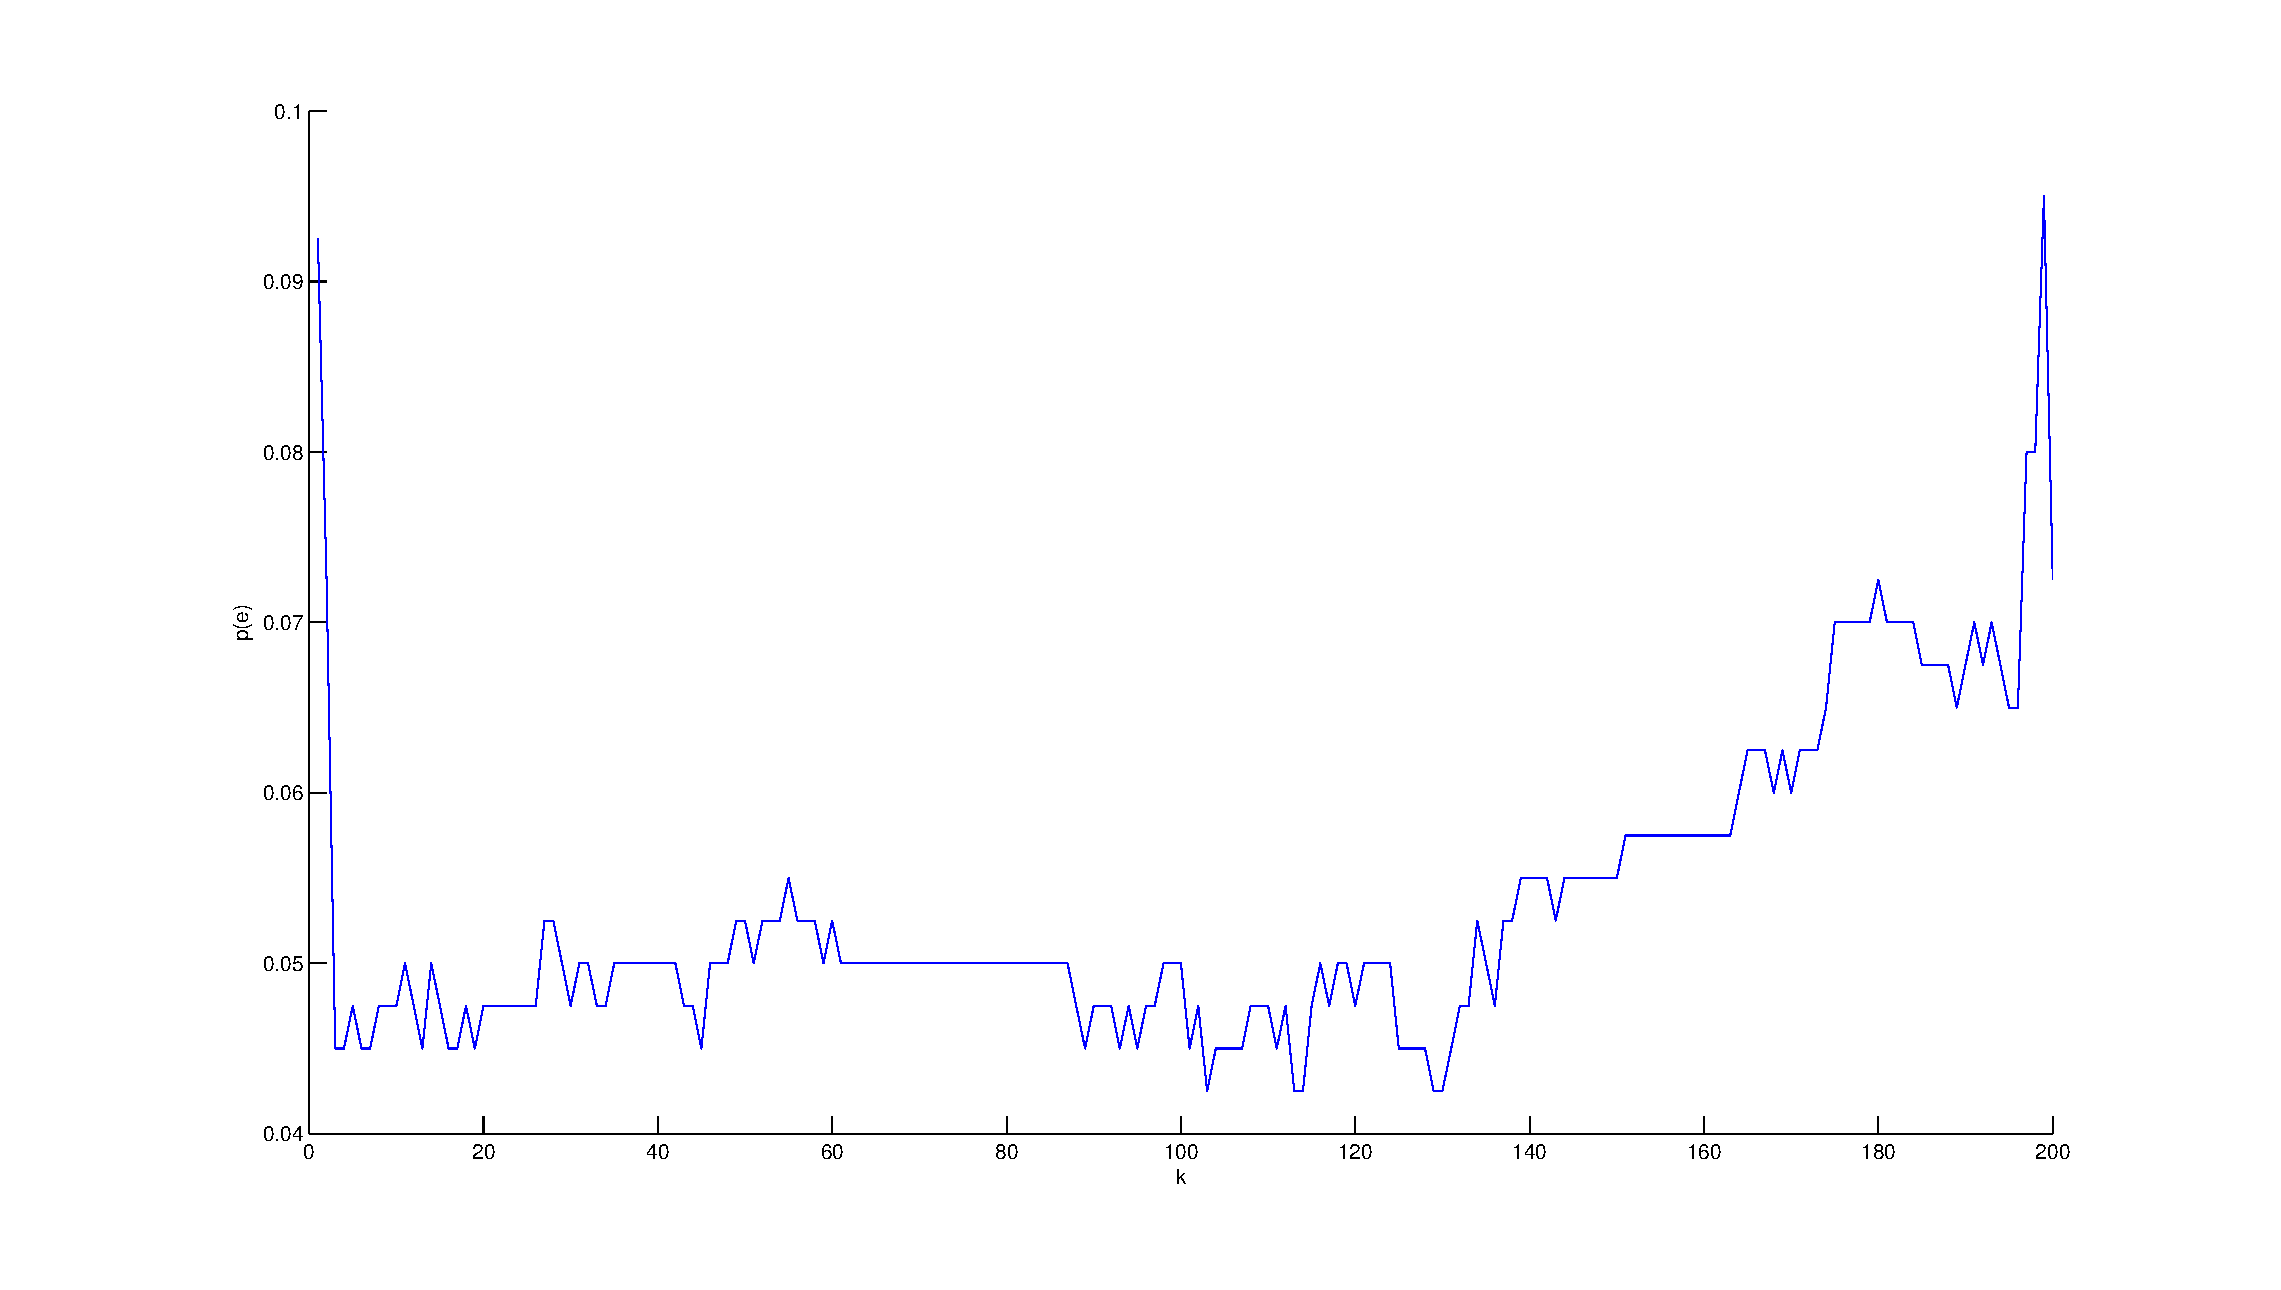
\includegraphics[width=15cm]{figures/2-err}
  \end{center}
\end{figure}

\begin{figure}
  \begin{center}
  	\label{fig:3err}  
    \caption{The probability of error as k increases for the 3 class case.}
    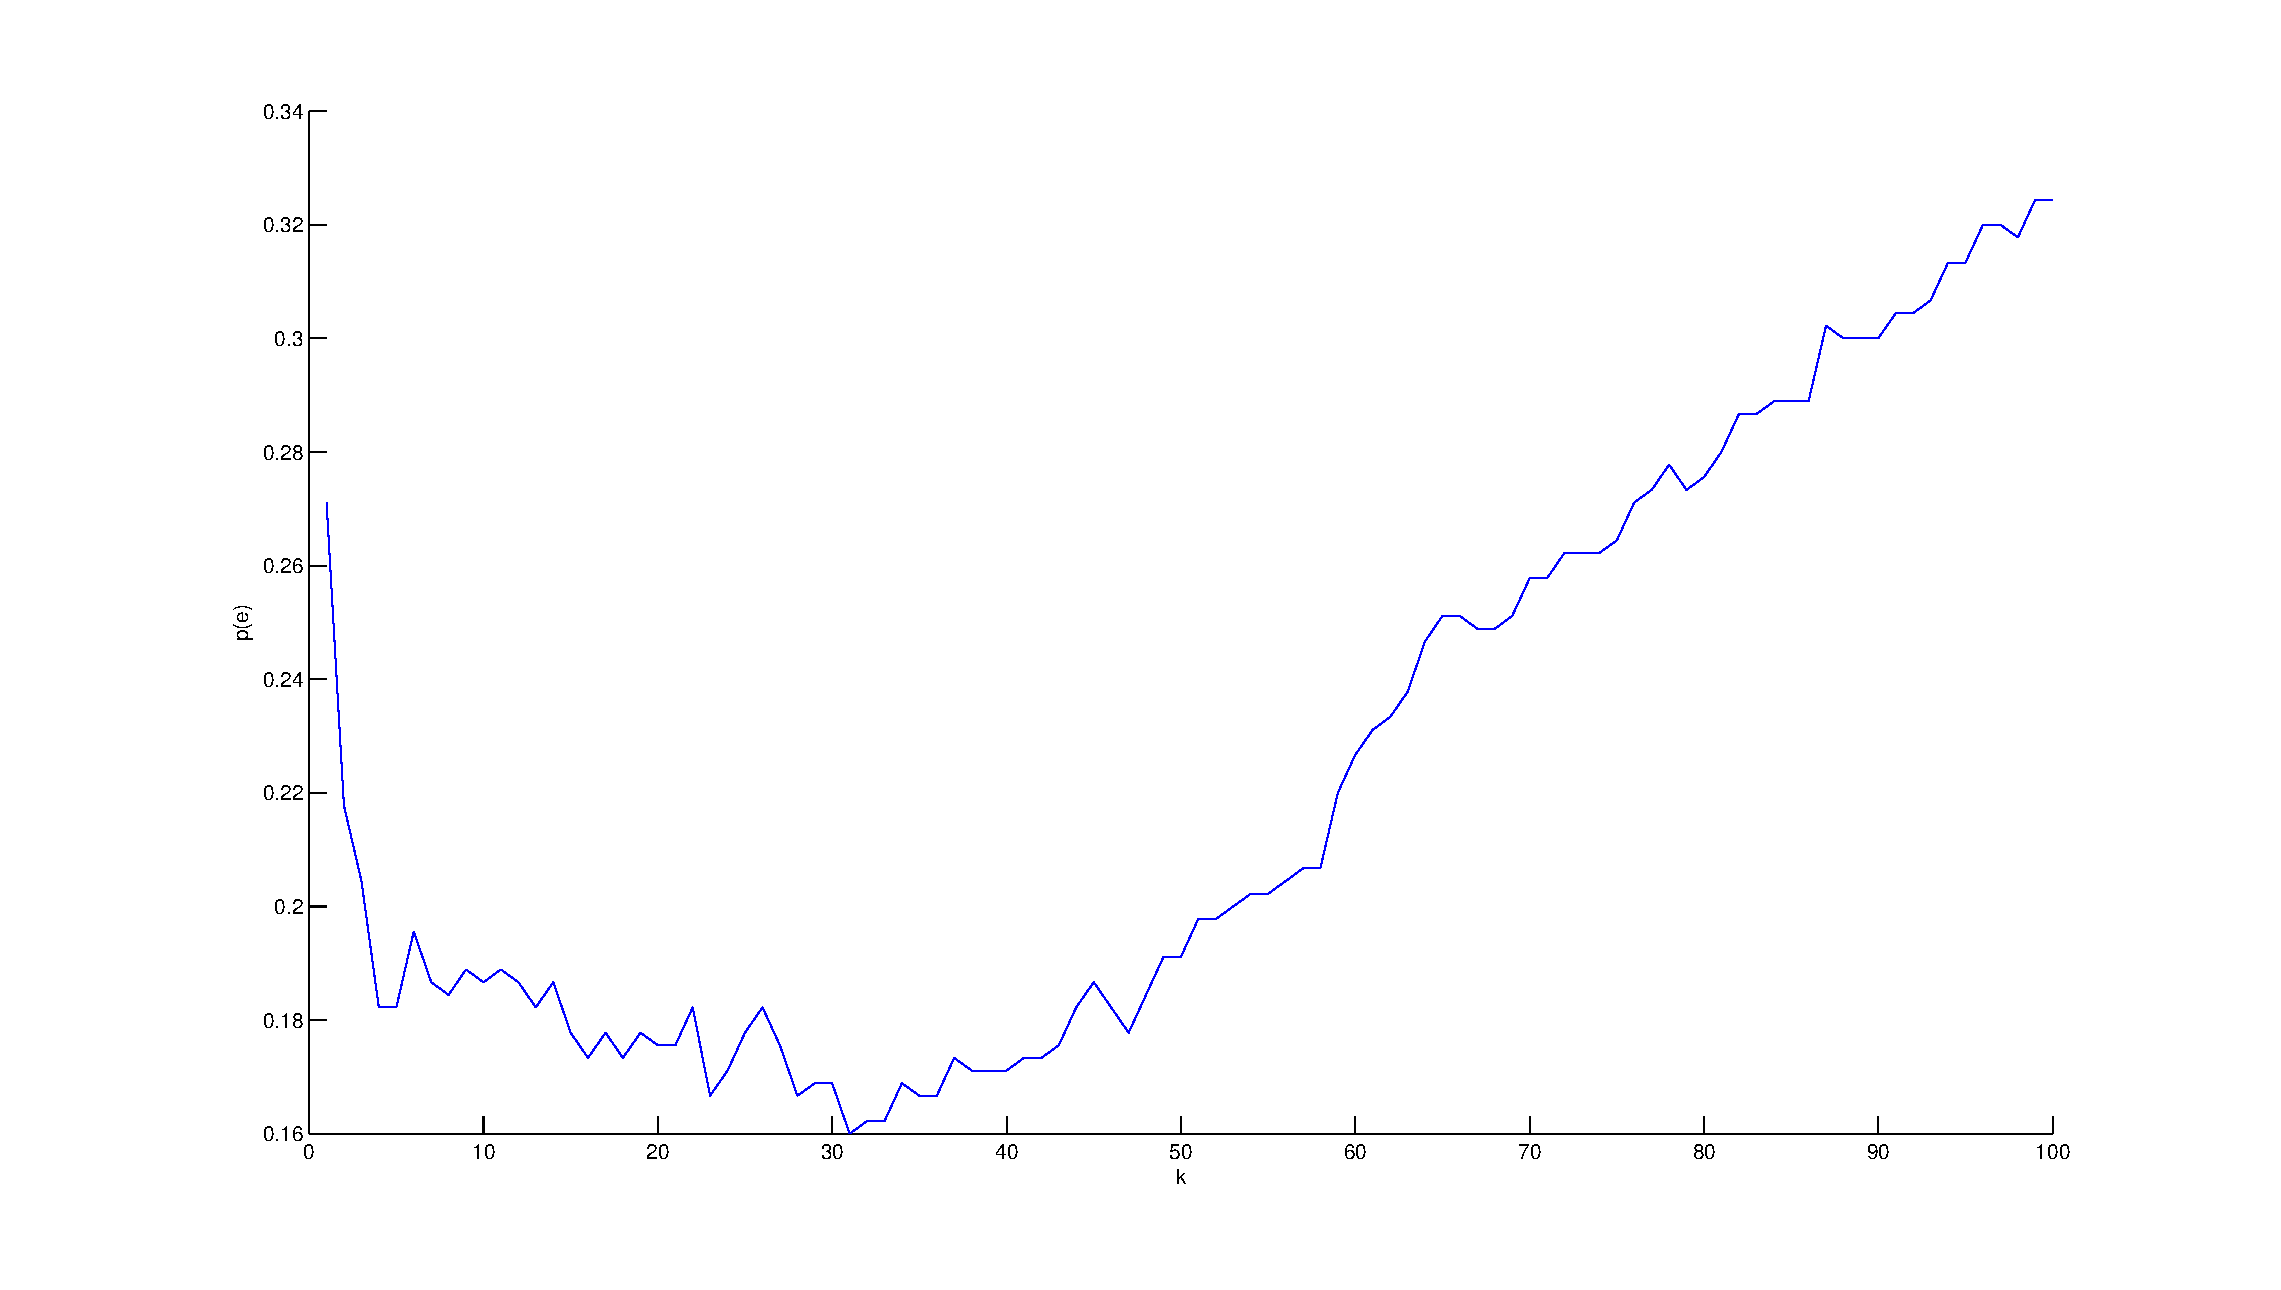
\includegraphics[width=15cm]{figures/3-err}
  \end{center}
\end{figure}

To explore the effect of the choice of k on the probability of error, a simple 
for loop was created to calculate the probability of error for the range 
of possible k ($0 < k < n_{smallest\_class}$). The graphs of a sample run of
this code are depicted in Figures \ref{fig:2err} and \ref{fig:3err} The graphs
generally show a sharp initial decrease as outliers are ignored. 
After the initial drop, the graphs tend to behave slightly differently for the
2- and 3-class cases.  For the 2-class case, the probability of error remains
relatively stable for the majority of the values of k, but begins to increase
as k approaches 75\% of its maximum value. For the 3-class case, however, it
seems that the probability of error begins to climb shortly following the
initial drop.  This suggests that class structure is eroded more quickly due to the exclusion of good data for the 3-class case.  From this result, we might suspect that this trend would
hold as the number of classes increases.

\chapter{Conclusions}
While MCID can provide better results, fuzzy classification is more flexible
and requires less input from the user.

The most important thing when using MCID classification of labelled data is to
have a large enough set of features. This is seen when the images are divided
into 2x2 matricies and the classification performs poorly.

\appendix
\renewcommand{\thechapter}{\Alph{chapter}}

\chapter{Code}
\label{cha:code}
\definecolor{grey}{rgb}{0.5,0.5,0.5}
\lstset{numbers=left, numberstyle=\tiny,language=Matlab,
basicstyle=\tiny, keywordstyle=\color{blue},
commentstyle=\color{grey},frame=single,breaklines=true}

\section{lab2p1.m}
\label{sec:lab2p1}
\lstinputlisting{../code/lab2p1.m}

\section{OneD.m}
\label{sec:oned}
\lstinputlisting{../code/OneD.m}

\section{lab2p2.m}
\label{sec:lab2p2}
\lstinputlisting{../code/lab2p2.m}

\section{TwoD.m}
\label{sec:twod}
\lstinputlisting{../code/TwoD.m}

\section{SequentialEstimation.m}
\label{sec:seq_est}
\lstinputlisting{../code/SequentialEstimation.m}

\end{document}  
